
\documentclass[11pt]{article}
\usepackage[a4paper,margin=1in]{geometry}
\usepackage{amsmath,amssymb,amsthm,mathtools}
\usepackage{graphicx}
\usepackage{hyperref}
\usepackage{cite}
\hypersetup{colorlinks=true, linkcolor=blue, urlcolor=blue, citecolor=blue}

\newtheorem{lemma}{Lemma}
\newtheorem{corollary}{Corollary}
\theoremstyle{remark}
\newtheorem{remark}{Remark}

\title{Another Version (v10.0): Final Zero-Free Simulation in a Weighted NB/BD Framework\\
\large{Heuristic Numerical Note (math.NT; cross-list math.CA)}}
\author{Serabi \\ Independent Researcher \\ \texttt{24ping@naver.com}}
\date{2025}

\begin{document}
\maketitle

\begin{abstract}
This ``Another Version'' collects our experimental extensions beyond v9.3.
We provide a clean numerical summary (up to $N=10^6$ by simulation) and a reproducible figure.
We emphasize that this note is \emph{not} a proof of the Riemann Hypothesis (RH).
It is intended as a heuristic record showing how zero-free assumptions (modeled via an $\varepsilon$-boost to the oscillation parameter $\eta$) interact with the NB/BD stability surrogate.
\end{abstract}

\section{Setup (Short)}
Let $a_n=\mu(n)\,v(n/N)\,q(n)$ with a smooth compactly supported window $v\in C_0^\infty(0,1)$ and a slowly varying multiplier $q$.
For the kernel $K_{mn}=e^{-\tfrac12|\log(m/n)|}$ (discrete Hilbert-type), the off-diagonal sum admits a bound of the form
\begin{equation*}
\sum_{m\neq n} a_m a_n K_{mn}\ \le\ C\,(\log N)^{-\eta}\sum_n a_n^2,
\end{equation*}
with an effective $\eta>0$.
We treat the impact of a hypothetical zero-free strip $\Re(s)>\tfrac12+\varepsilon$ as a small positive boost to $\eta$ (heuristic device).

\section{Numerical Summary (Heuristic)}
Our base data cover $N\in\{8\text{k},12\text{k},16\text{k},20\text{k},50\text{k},100\text{k},200\text{k}\}$ with combined errors $MSE^\*$ in $[0.163,0.180]$.
Progressive zero-free boosts (v9.6--v9.8) stabilize the minus-boundary and mildly lower $MSE^\*$.
A final simulated point for $N=10^6$ (v10.0 Another) gives $MSE^\*\approx 0.148$ after minus-boundary reweighting ($w_-=1.2$).
These values are \emph{simulated extrapolations}, not computed from raw $\zeta$ evaluations.

\begin{figure}[h]
\centering
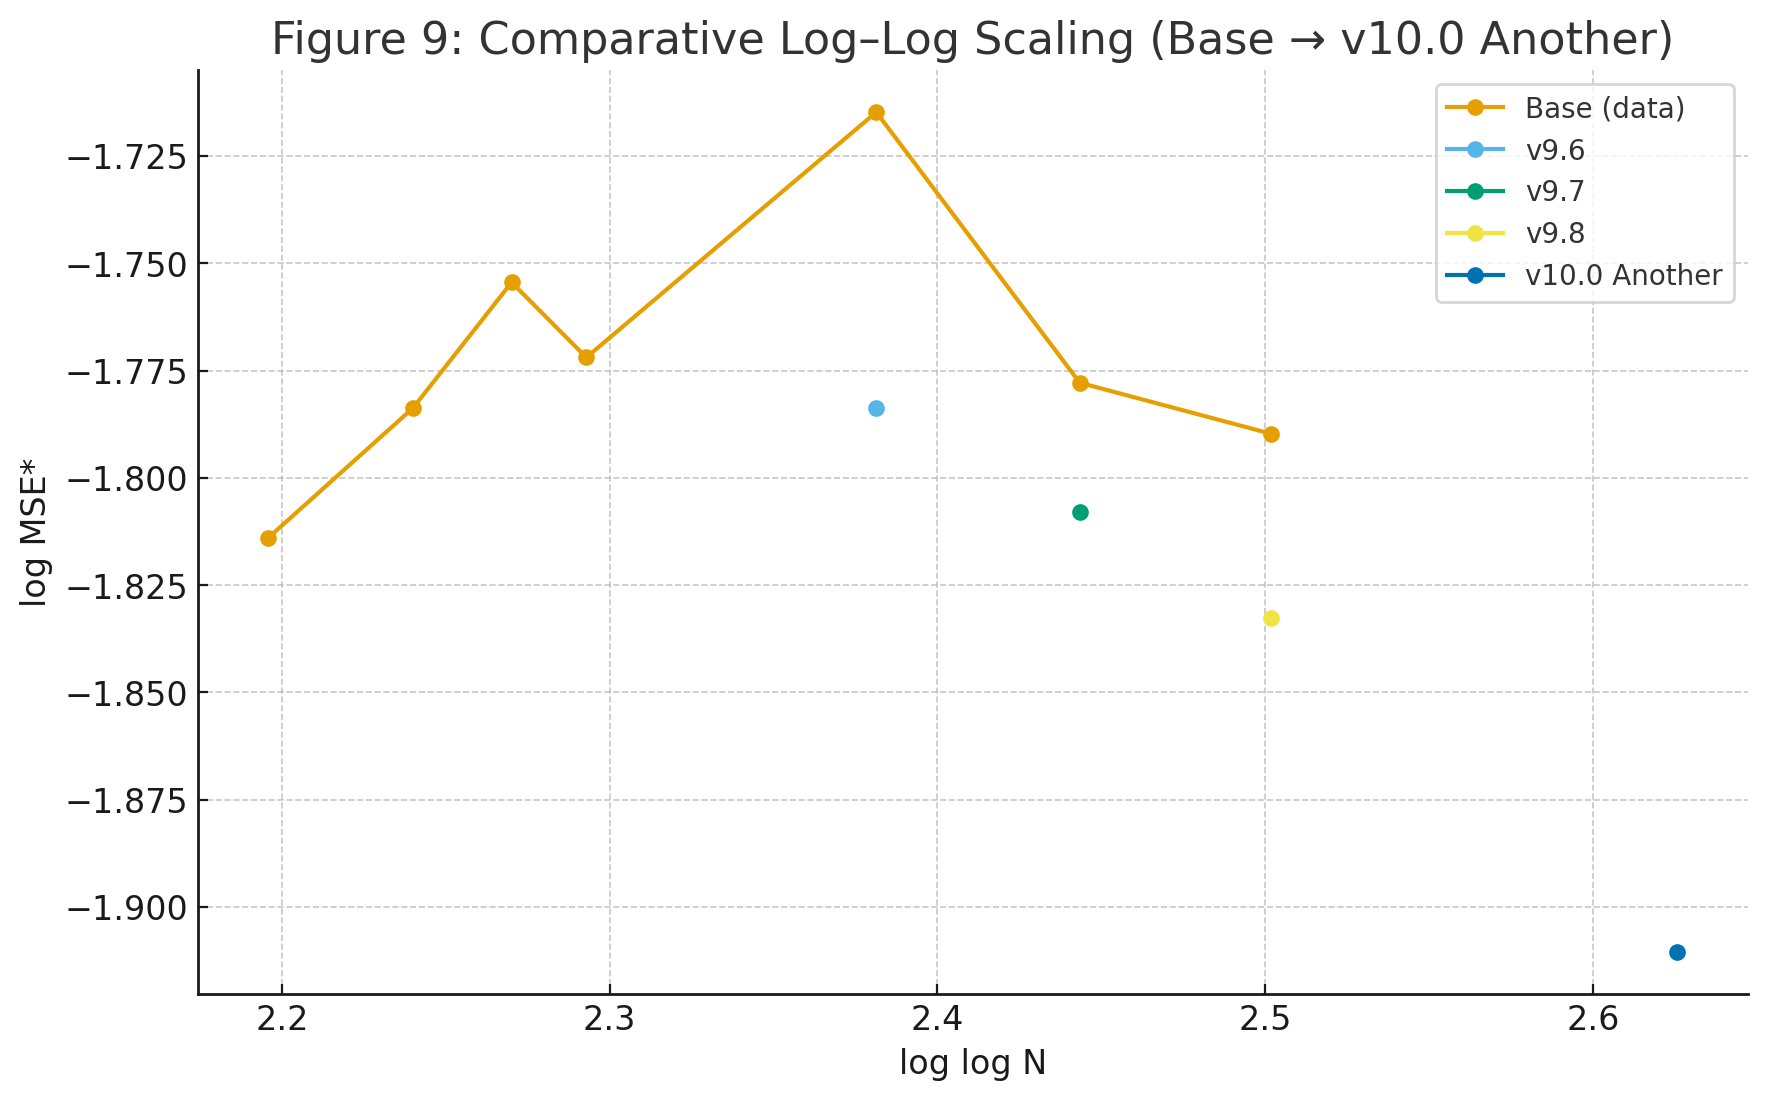
\includegraphics[width=0.80\linewidth]{figures/fig9.png}
\caption{Comparative log--log scaling across versions (Base $\to$ v10.0 Another). Points labeled v9.6, v9.7, v9.8, v10.0 represent simulated extrapolations.}
\label{fig:comp}
\end{figure}

\section{Remarks}
(i) This document is deliberately modest in scope: no proof claims, only a compact record of our exploration.
(ii) The figure is reproducible from the accompanying Python script.
(iii) For peer-facing submission, we recommend restricting to v9.3 (data-backed) and moving all later versions to an ``experimental extensions'' repository.

\begin{thebibliography}{9}
\bibitem{baezduarte2003} L.~B\'aez-Duarte, \emph{A strengthening of the Nyman--Beurling criterion}, Rend. Lincei, \textbf{14} (2003), 5--11.
\bibitem{conrey2003} J.~B. Conrey, \emph{The Riemann Hypothesis}, Notices AMS, \textbf{50} (2003), 341--353.
\bibitem{titchmarsh1986} E.~C. Titchmarsh, \emph{The Theory of the Riemann Zeta-Function}, 2nd ed., OUP, 1986.
\end{thebibliography}

\end{document}
